% Created 2017-08-31 Thu 02:25
% Intended LaTeX compiler: pdflatex
\documentclass[11pt]{article}
\usepackage[utf8]{inputenc}
\usepackage[T1]{fontenc}
\usepackage{graphicx}
\usepackage{grffile}
\usepackage{longtable}
\usepackage{wrapfig}
\usepackage{rotating}
\usepackage[normalem]{ulem}
\usepackage{amsmath}
\usepackage{textcomp}
\usepackage{amssymb}
\usepackage{capt-of}
\usepackage{hyperref}
\usepackage{amsthm}
\usepackage{amsmath}
\usepackage{tikz-cd}
\newtheorem{remark}{Remark}
\newtheorem{theorem}{Theorem}
\newtheorem{lemma}[theorem]{Lemma}
\newtheorem{corollary}{Corollary}[theorem]
\newtheorem{conjecture}[theorem]{Conjecture}
\newtheorem{proposition}{Proposition}[theorem]
\newtheorem{problem}{Problem}
\newtheorem{exampl}{Example}
\newtheorem{definition}{Definition}
\newtheorem{propdef}[definition]{Proposition-Definition}
\newcommand{\im}{\mathop{\rm Im}\nolimits}
\newcommand{\supp}{\mathop{\rm supp}\nolimits}
\newcommand{\ord}{\mathop{\rm ord}\nolimits}
\author{darknmt}
\date{\today}
\title{Sheaves and Cohomology}
\hypersetup{
 pdfauthor={darknmt},
 pdftitle={Sheaves and Cohomology},
 pdfkeywords={},
 pdfsubject={},
 pdfcreator={Emacs 25.2.1 (Org mode 9.0.5)}, 
 pdflang={English}}
\begin{document}

\maketitle
\tableofcontents

\iffalse
\begin{info}
The PDF version of this page can be downloaded by replacing \texttt{html} in the its address by
\texttt{pdf}. 
For example \texttt{/html/sheaf-cohomology.html} should become \texttt{/pdf/sheaf-cohomology.pdf}.
\end{info}
\fi


\section{Sheaf and Presheaf}
\label{sec:org89ea00e}
\begin{definition}
Let \(M\) be a manifold, a \textbf{sheaf} over \(M\) is a couple \((\mathcal{S}, \pi)\) with \(\mathcal{S}\) a topologized space and \(\pi: \mathcal{S}\longrightarrow M\) a \uline{local
homeomorphism} such that each \textbf{stalk} \(\pi^{-1}(m)\) is a \(R\)-module.

A \textbf{presheaf} is a way to associate each open set \(U\subset M\) a \(R\)-module \(\mathcal{S}(U)\) and morphisms \(\iota_{V,U}: \mathcal{S}(U) \longrightarrow
\mathcal{S}(V)\) which satisfy cocycle condition.
\end{definition}

\begin{remark}
\begin{enumerate}
\item In spirit, by \uline{taking section} and \uline{taking germ} (direct limit) the two objects are the
same. Technically, in order to obtain an equivalent condition, one has to restrict to
presheaves that satisfy: For every covering \(\{U_i\}\) of \(U\)
\begin{enumerate}
\item \(f=g\) in \(\mathcal{S}(U)\) if and only if \(\iota_{U_i, U} f = \iota_{U_i, U} g\) for every \(i\).
\item For every family \(f_i \in \mathcal{S}(U_i)\) that satisfies \(\iota_{U_i\cap
      U_j, U_i}f_i = \iota_{U_j\cap U_i, U_j}f_j\) there exists an \(f \in
      \mathcal{S}(U)\) such that \(\iota_{U_i,U} f = f_i\).
\end{enumerate}
\item Usual operation on modules can be extend to sheaves. The tensor product, for example,
can be defined on presheaves then pass to sheaves (in order not to deal with the
topology)
\end{enumerate}
\end{remark}

\section{Cohomology of complexes}
\label{sec:orgbad4845}

\subsection{Construction and naturality}
\label{sec:orgdb74180}
  A \textbf{complex} is a sequence \(C_0 \longrightarrow C_1 \longrightarrow \dots \longrightarrow C_n
\longrightarrow \dots\) such that the composition of two consecutive arrows vanishes. The
cohomology \(H^n(C_*)\) is defined by \(H^n(C_*) = \ker d_{n}/ \im d_{n-1}\).

Then \href{https://en.wikipedia.org/wiki/Snake\_lemma}{Snake lemma} implies

\begin{theorem}[Long exact sequence + Naturality]
\label{thm:cohomology-complex}
If \(0 \longrightarrow  C_* \longrightarrow D_* \longrightarrow E_* \longrightarrow 0\)
is a \textbf{short exact sequence of complexes}, then one has
\begin{enumerate}
\item Long exact sequence:
\[\dots \longrightarrow  H^n(C_*) \longrightarrow  H^n(D_*) \longrightarrow H^n(E^*) \longrightarrow
   H^{n+1}(C^*) \longrightarrow \dots \]
\item Any morphism between short exact sequences gives rise to a morphism between long exact sequences.
\end{enumerate}
\end{theorem}

\begin{verbatim}
\begin{tikzcd}
  0 \ar[d] & 0 \ar[d] \\
  C_* \ar[d] \ar[r] & C'_* \ar[d] \\
  D_* \ar[d] \ar[r] & D'_* \ar[d] \\
  E_* \ar[d] \ar[r] & E'_* \ar[d] \\
  0 & 0 
\end{tikzcd}\quad 
\begin{tikzcd} 
  H^n(C_*) \ar[d] \ar[r] & H^n(D_*) \ar[d] \ar[r] & H^n(E_*) \ar[r] \ar[d] & H^{n+1}(C_*) \ar[d] \\
  H^n(C'_*) \ar[r] & H^n(D'_*) \ar[r] & H^n(E'_*) \ar[r] & H^{n+1}(C'_*) 
\end{tikzcd}
%\caption{Morphism between short exact sequences gives rise to a morphism between long exact sequences.}
\label{fig:morph-short-sequence}
\end{verbatim}


\begin{figure}[htbp]
\centering
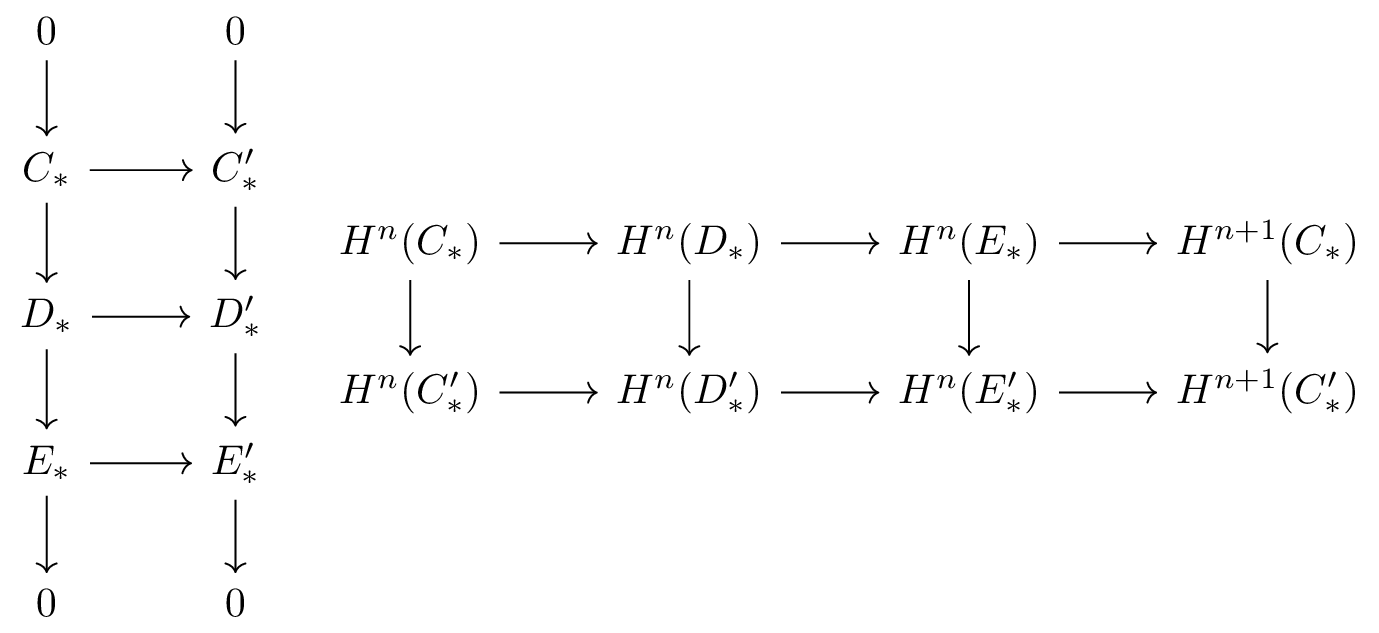
\includegraphics[width=1.0\textwidth]{../img/2017-08-13-morph-short-sequence.png}
\caption{Morphism between short exact sequences gives rise to a morphism between long exact sequences. [fig:morph-short-sequence]}
\end{figure}


The algebraic machinery behind \href{http://mathworld.wolfram.com/PoincaresLemma.html}{Poincaré lemma} is the following

\begin{theorem}[Homotopy/Prism operator]
\label{thm:prism-operator}
Let \(f\) and \(g\) be two morphism between complexes \(\{C_*\}, \{D_*\}\) such that there
exists a diagonal morphism \(\epsilon:  C_n \longrightarrow  D_{n-1}\) that satisfies
\(f-g = d_D \circ \epsilon = \epsilon \circ d_C\) then \(f\) and \(g\) induce the same
morphism from \(H^n(C_*)
\longrightarrow  H^n(D_*)\).
\end{theorem}

\begin{verbatim}
\begin{tikzcd}
  C_{n-1} \ar[d] \ar[r] & D_{n-1} \ar[d] \\
  C_n \ar[d] \ar["\varepsilon", ur] \ar["f-g", r] & D_n \ar[d] \\
  C_{n+1} \ar["\varepsilon", ur] \ar[r] & D_{n+1} 
\end{tikzcd}
%\caption{Homotopy operator \( \varepsilon \).}
\label{fig:homotopy-operator}
\end{verbatim}


\begin{figure}[htbp]
\centering
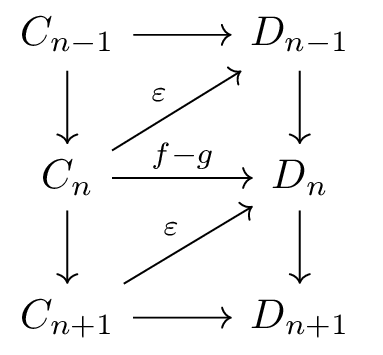
\includegraphics[width=0.30\textwidth]{../img/2017-08-13-homotopy-operator.png}
\caption{Homotopy operator \(\varepsilon\). [fig:homotopy-operator].}
\end{figure}

\subsection{Multiplicative structure}
\label{sec:org2db2961}
Given two complexes \(\{C_*\},\{D_*\}\), one can define their tensor product as \(E_* =
C_* \otimes D_*\) with
\[
0 \longrightarrow C_0\otimes D_0 \longrightarrow (C_0\otimes D_1) \oplus (C_1\otimes D_0)
\longrightarrow \dots
\]
with the tensor coboundary \(d_E = d_C\otimes1 + (-1)^p\otimes d_D\) where \(p\) is the
degree of the \$C\$-components. One then has the following algebraic result
\begin{theorem}[Künneth]
\label{thm:Kunneth}
If \(R\) is a field then one has the following decomposition
\[
 \oplus_k \left( H^k\left(C_*\right) \otimes_k H^{n-k}\left(D_*\right)
 \right) \stackrel{\simeq}{\to} H^n\left( C_* \otimes_k D_* \right) 
\]
\end{theorem}



\section{Axiomatic cohomology theory}
\label{sec:org62ef2d8}
Let \(M\) be a manifold, a \textbf{cohomology theory} on \(M\) is a \uline{functor} from the \uline{category of
sheaves over \(M\)} to the \uline{category of graded \(R\)-module} such that
\begin{enumerate}
\item Each sheaf \(\mathcal{S}\) corresponds to a graded module sequence \(H^n(M,\mathcal{S})\) with \(H^0(M,\mathcal{S}) = \Gamma(S)\) the module of global
sections of \(\mathcal{S}\) and \(H^{n}(M, \mathcal{S}) = 0\) if \(n<0\). Morphisms between sheaves are transformed to morphisms between cohomology.
\item Any short exact sequence \(0 \longrightarrow \mathcal{S}' \longrightarrow \mathcal{S}
   \longrightarrow \mathcal{S}'' \longrightarrow 0\) gives rise to a long exact sequence
\[
   \dots \longrightarrow H^n(M, \mathcal{S}') \longrightarrow H^n(M, \mathcal{S}) \longrightarrow H^n(M,
   \mathcal{S}'') \longrightarrow H^{n+1}(M, \mathcal{S}') \longrightarrow \dots
   \] 
One also has the naturality for such long sequence, i.e. for the coboundary map \(H^n(M, \mathcal{S}'') \longrightarrow H^n(M, \mathcal{S}')\).
\item Cohomology of a fine sheaf is 0.
\end{enumerate}

A sheaf \(\mathcal{S}\) is called \textbf{fine} if for every locally finite open cover \(U_i\) of \(M\), there exists automorphisms \(f_i\) of \(\mathcal{S}\) such that \(\supp f_i \subset U_i\) and \(\sum f_i = Id_\mathcal{S}\).


\subsection{Existence and Uniqueness}
\label{sec:org65911e0}
The next theorem will give a cohomology theory given that one has a \textbf{resolution}, i.e. an
exact sequence 
\[
0 \longrightarrow K \longrightarrow \mathcal{C}_0 \longrightarrow
\mathcal{C}_1 \longrightarrow \dots 
\] 
where \(K\) is the constant sheaf \(M\times R\). Such a resolution does exist, the most
natural one may be the de Rham resolution, which gives de Rham cohomology that we will
discuss later. 

\begin{theorem}[Existence of cohomolgy theory]
\label{thm:existence-cohomology}
Let \(\mathcal{C}_*\) be a resolution of \(M\), then the cohomology of the following
complex
\[
0 \longrightarrow \Gamma(\mathcal{C}_0 \otimes \mathcal{S}) \longrightarrow
\Gamma(\mathcal{C}_1 \otimes \mathcal{S}) \longrightarrow \dots
\]
for an arbitary sheaf \(\mathcal{S}\) is a cohomology theory.
\end{theorem}

It worths mentioning that the intuition behind such construction is the half-exactness of
operations \(\mathcal{A} \mapsto \mathcal{A}\otimes \mathcal{S}\) and \(\mathcal{A}\mapsto \Gamma(A)\). For example, one can show, using the following exactness,
that fine sheaves are of trivial cohomology.

\begin{lemma}[]
\label{lem:exactness}
\begin{enumerate}
\item "Tensoring" functor is right exactness, i.e. a short exact sequence \(0 \longrightarrow
   \mathcal{C}' \longrightarrow \mathcal{C} \longrightarrow \mathcal{C}'' \longrightarrow
   0\) induces
\[
   \mathcal{C}'\otimes \mathcal{T} \longrightarrow \mathcal{C}\otimes \mathcal{T}
   \longrightarrow \mathcal{C}''\otimes \mathcal{T} \longrightarrow 0.
   \]
Moreover, if \(\mathcal{C}''\) or \(\mathcal{T}\) is torsionless, one has
\[
   0 \longrightarrow \mathcal{C}'\otimes \mathcal{T} \longrightarrow \mathcal{C}\otimes \mathcal{T}
   \longrightarrow \mathcal{C}''\otimes \mathcal{T} \longrightarrow 0.
   \]
\item \(\Gamma\) fuctor is left exact, i.e. a short exact sequence \(0 \longrightarrow
   \mathcal{C}' \longrightarrow \mathcal{C} \longrightarrow \mathcal{C}'' \longrightarrow
   0\) induces
\[
   0 \longrightarrow \Gamma(\mathcal{C}') \longrightarrow \Gamma(\mathcal{C}) \longrightarrow \Gamma(\mathcal{C}'').
   \]
Moreover, if \(\mathcal{C}'\) is fine then
\[
   0 \longrightarrow \Gamma(\mathcal{C}') \longrightarrow \Gamma(\mathcal{C})
   \longrightarrow \Gamma(\mathcal{C}'') \longrightarrow 0.
   \]
\item If \(\mathcal{S}\) or \(\mathcal{T}\) is fine, then \(\mathcal{S}\otimes
   \mathcal{T}\) is fine.
\end{enumerate}
\end{lemma}


One might note that such a cohomology depends a priori on the resolution \(\mathcal{C}_*\), the following result claims that in fact any resolution gives the same theory.

\begin{theorem}[Uniqueness of cohomology theory]
\label{thm:uniqueness-cohomology}
Any two cohomology theory \(\mathcal{H}, \tilde{\mathcal{H}}\) has \(\#Func(\mathcal{H},
\tilde{\mathcal{H}}) =1\), therefore the two are naturally isomorphic.
\end{theorem}

It is straight-forward to see that the computation of cohomology is much simplified if one
can find a \textbf{fine resolution} \(\mathcal{C}_n\) of \(\mathcal{S}\), i.e. fine sheaves
\(\mathcal{C}_n\) such that \(0 \longrightarrow \mathcal{S}\longrightarrow
\mathcal{C}_0 \longrightarrow \mathcal{C}_1 \longrightarrow \dots\)

\begin{theorem}[]
\label{thm:fine-resolution}
If  \(0 \longrightarrow \mathcal{S}\longrightarrow
\mathcal{C}_0 \longrightarrow \mathcal{C}_1 \longrightarrow \dots\) is a fine resolution
of \(\mathcal{S}\) then
\[
H^n(M, \mathcal{S}) = \Gamma(\mathcal{C}_n)
\]
\end{theorem}

\begin{remark}
\sout{A consequence of uniqueness of cohomology theory is the following.} From the construction
in Theorem \ref{thm:existence-cohomology}, given a sheaf \(\mathcal{S}\) of \(R_2\)module and \(R_1\) is a subring of \(R_2\) then the
cohomology \(H^*(M, \mathcal{S})\) of \(\mathcal{S}\) can be defined in the category
of \(R_1\)-sheaves or \(R_2\)-sheaves, noted by the \(R_i\)-modules \(H^*(M,
\mathcal{S})_{R_i}\). Then \(H^*(M, \mathcal{S})_{R_2}\) is isomorphic to \(H^*(M,
\mathcal{S})_{R_1}\) as \(R_1\)-modules.

By this reason, the base ring \(R\) is not expressed explicitly in the notation \(H^*(M, \mathcal{S})\).
\end{remark}


\subsection{Multiplicative structure}
\label{sec:org35048ea}

If each stalk \(\mathcal{S}(x)\) is more than an \(R\)-module but an \(R\)-algebra, then one can endow \(H^n(M, \mathcal{S})\) with a multiplicative structure
that it a graded algebra. This structure come from the tensor product of the complex \(\Gamma(\mathcal{C}_n\otimes S)\) with itself and from the natural inclusion
\[
\Gamma(\mathcal{C}_p\otimes\mathcal{S}) \otimes \Gamma(\mathcal{C}_q\otimes\mathcal{S})
\longrightarrow \Gamma(\mathcal{C}_{p+q} \otimes \mathcal{S}).
\]
which give \(H^p(M,\mathcal{S})\otimes H^q(M, \mathcal{S}) \longrightarrow H^{p+q}(M,
\mathcal{S})\).


\subsection{Examples: de Rham cohomology}
\label{sec:orgbd2adbd}
Taking \(\mathcal{C_n} = \Omega^n(M)\) the sheaves of germs of \(n\)-forms on \(M\), then by Theorem \ref{thm:fine-resolution} one obtains the \textbf{de Rham cohomology} \(H^n(M,
  \mathbb{R}\). By the same way, one can construct \textbf{Alexander–Spanier cohomology} and
\textbf{singular cohomology}.

\begin{theorem}[de Rham]
\label{thm:de-rham-singular}
The unique natural transformation from de Rham cohomology to singular cohomology is given
by \(\omega_n \mapsto \left(\Delta_n \mapsto \int_{\Delta_n}\omega_n \right)\) and sends
the wedge product in de Rham cohomology to cup-product in singular cohomology.
\end{theorem}

\section{Čech cohomology}
\label{sec:org91022b2}
Čech cohomology is another important cohomology whose construction is not based on a
resolution. Čech cohomology \(\check{H}(M, \mathcal{S})\) is defined as the direct limit
of the following \(\check{H}(M,\mathcal{S},\mathcal{U})\) when \(\mathcal{U}\) becomes
finer as an open cover of \(M\).

Let \(\mathcal{U}\) be an open cover of \(M\). A \(n\)-cocyle in \(C_{n,\mathcal{U}}\) is defined as a
mapping 
\[ 
\sigma: (U_0,\dots, U_n) \mapsto \sigma(U_0,\dots, U_n) \in \mathcal{S}\left(\cap_{i=0}^n
U_i\right)
\]
and the coboundary \(d\sigma \in C_{n+1,\mathcal{U}} : (U_0,\dots, U_{n+1}) \mapsto
\sum_i \iota_{\cap U_i}(-1)^i
\sigma (U_0,\dots,\check{U_i},\dots, U_{n+1})\). The cohomology of this complex is noted
as \(\check{H}^*(M, \mathcal{S},\mathcal{U})\).

\begin{remark}
Let \(\mathcal{V}\) be a finer cover of \(M\), i.e. every open \(V_i\) in \(\mathcal{V}\) is included in an element \(U_{j_i}\) of \(\mathcal{U}\), there exists
a natural map \(\check{H}^*(M, \mathcal{S},\mathcal{V}) \longrightarrow \check{H}^*(M,
\mathcal{S},\mathcal{U})\) induced by the \(C_{n,\mathcal{V}} \longrightarrow
C_{n,\mathcal{U}}\) which depends on the refining map \(j\). Using Theorem
\ref{thm:prism-operator}, one can prove that the induced map between cohomology is however
independent of \(j\).
\end{remark}


\subsection{Example: Picard group}
\label{sec:org9316080}
Let \(X\) be a complex manifold. A vector bundle of \(X\) is called \textbf{holomorphic}
iff the projection map is holomorphic. 
\begin{remark}
A holomorphic vector bundle is different from a vector bundle with holomorphic transition
functions. In 1 dimension for example, an (differential) isomorphic class of line bundle with holomorphic
transition can be encoded as an element of \(H^1(X, \mathbb{C})\). Meanwhile, an
(complex) isomorphic class of holomorphic line bundle is an element of \(H^1(X, \mathcal{O}^*)\).
\end{remark}


\begin{definition}
The \textbf{Picard group} \(\text{Pic}(X)\) is the commutative group of holomorphic line
bundles over \(X\) with the tensor product. Another way to regard \(\text{Pic}(X)\) is
by \(\text{Pic}(X) = \check{H}^1(X, \mathcal{O}^*)\).
\end{definition}




\subsection{Example: first Chern class in \(H^2(X, \mathbb{Z})\)}
\label{sec:orgd0b07bb}
   The following short exact sequence of \(\mathbb{Z}\)-module
\[
0 \longrightarrow \mathbb{Z} \longrightarrow \mathcal{O}_X \longrightarrow \mathcal{O}_X^*
\longrightarrow 0
\]
gives the long exact sequence:
\[
H^1(X, \mathcal{O}_X) \longrightarrow H^1(X, \mathcal{O}_X^*) \longrightarrow H^2(X,
\mathbb{Z}) \longrightarrow \dots
\]
Since \(H^1(X, \mathcal{O}_X^*)\) is Picard group, the \uline{first Chern class} \(c_1(L)\) of a
holomorphic line bundle \(L\) is the image of \(L\) in \(H^2(X, \mathbb{Z})\).

\subsection{Example: from divisor to Picard group}
\label{sec:org6924367}

An \textbf{analytic subvariety} \(Y\) of a complex manifold \(X\) is a closed set such that
locally at each \(y\in Y\), \(Y\) is zero of a holomorphic function.

\begin{remark}
A analytic hypersurface \(Y\) can be completely encoded by a family \(( U_i, f_i)\)
where \(f_i\) is a meromorphic function on \(U_i\) with \(U_i\cap Y\) its zeros. The
latter is a global section of \(H^1(X, K^*_X/ \mathcal{O}^*_X)\) where \(K_X^*\)
denotes the sheaf of meromorphic germs that is not the zero germ and \(\mathcal{O}_X^*\)
denotes the sheaf of holomorphic germs that is non-zero \uline{at every point}
(invertible). These are sheaves of \(\mathbb{Z}\)-modules.
\end{remark}

This correspondance is not one-to-one, as \(2.s = s^2 \in H^1(X, K^*_X/\mathcal{O}_X^*)\) describe the same hypersurface. This phenomenon can be avoid with the notion of
divisor.

\begin{definition}
An \textbf{irreducible hypersurface} of \(X\) is a analytic hypersurface that is not union of
smaller analytic hypersurfaces.

A \textbf{divisor} \(D\) on \(X\) is a formal sum \(D = \sum a_i Y_i\) where \(a_i\in
\mathbb{Z}\) and \(Y_i\) is an irreducible hypersurface. \(D\) is called \textbf{effective}
if and only if \(a_i \geq 0\).

Let \(f\) be a meromorphic function on \(X\), the \textbf{principal divisor} associated to \(f\) is defined by \((f) = \sum \ord_{f,Y}Y\) where \(\ord\) denotes the order of \(f\) on an irreducible hypersurface \(Y\)
\end{definition}

Note that an irreducible hypersurface \(Y\) does not necessarily induce irreducible
germs in every point, but only almost all points (denoted by \(Y_{reg}\)). Therefore, one
can still define the order \(ord_{f,Y}\) of a meromorphic function \(f\) on \(Y\) as
the order in any regular points.

The next theorem follows immediately from the above discussion.
\begin{theorem}[Divisor-Line bundle relation]
\label{thm:div-pic-rel}
\begin{enumerate}
\item Given a divisor \(D = \sum a_i Y_i\), there exists a unique (isomorphic class of)
holomorphic line bundle \(L = \mathcal{O}(D)\) such that \(D =Z(s) = \sum \ord_{s,Y} Y\), the zero with
multiple of \(s\), where \(s\) a global section of \(L\). Given an open cover \(U_i\) fine enough, this line bundle is defined such that the functions \(s_i = \prod
   f_j^{\alpha_j}\) where \(Y_j = Z(f_j)\) in \(U_i\) form a global section.
\item On the other hand, given a line bundle \(L\) and any global section \(s\), there
exists a divisor \(D\) such that \(L = \mathcal{O}(D)\).
\item One has group morphism \(\text{Div}(X) \longrightarrow \text{Pic}(X)\) whose kernel
is the subgroup of principal divisors and every \(L\in \text{Pic}(X)\) with a
nontrivial global section is image of an effective divisor.
\end{enumerate}
\end{theorem}

The morphism \(\text{Div}(X) \longrightarrow \text{Pic}(X)\) can also be constructed by
the following short exact sequence
\[
0 \longrightarrow \mathcal{O}_X^* \longrightarrow K_X^* \longrightarrow K_X^*/
\mathcal{O}_X^* \longrightarrow 0
\]
which gives the long exact sequence
\[
H^0(X,K_X^*) \longrightarrow \text{Div}(X) = H^0(K_X^*/\mathcal{O}_X^*) \longrightarrow
H^1(X, \mathcal{O}_X^*) = \text{Pic}(X) \longrightarrow \dots
\]
This shows clearly that the kernel of the above group morphism is the group of principal divisors.
Emacs 25.2.1 (Org mode 9.0.5)
\end{document}